\chapter{Simulaci\'on de flujo multif\'asico}

\section{Lattice Boltzmann para flujo multif\'asico}
En sinton\'ia con el crecimiento de la mec\'anica de fluidos computacional, fueron desarroll\'andose numerosos m\'etodos num\'ericos macrosc\'opicos destinados a resolver las ecuaciones de Navier-Stokes en flujos multif\'asicos \cite{scardovelli_direct_1999}. Entre los m\'etodos m\'as populares, pueden destacarse el de \textbf{front-tracking}, el m\'etodo Volume of Fluid (VOF) y el m\'etodo level set. A pesar de la amplia difusi\'on adquirida, y de la demostrada capacidad para resolver con precisi\'on diversos escenarios con flujos multif\'asicos, estas t\'ecnicas tradicionales contin\'uan presentando limitaciones que dificultan el modelado de problemas complejos con transferencia de calor, como ebullici\'on y condensaci\'on. En particular, el m\'etodo de \textbf{front-tracking} generalmente no permite simular adecuadamente procesos de coalescencia y ruptura de una interfase \cite{scardovelli_direct_1999,liu_three-dimensional_2012}. La aplicaci\'on de VOF y level set suele requerir pasos de reconstrucci\'on o reinicializaci\'on de la interfase, que pueden no ser f\'isicos y complejos de implementar \cite{liu_three-dimensional_2012}. Adem\'as, suelen originarse inestabilidades num\'ericas en el uso de VOF o level set para simular flujos dominados por tensi\'on superficial en geometr\'ias complejas \cite{scardovelli_direct_1999}.
\par
En comparaci\'on con otros m\'etodos computacionales, el MLB presenta ventajas adicionales para la simulaci\'on de flujos complejos. Por un lado, la naturaleza mesosc\'opica con base en la teor\'ia cin\'etica molecular permite generar modelos con s\'olidos fundamentos termodin\'amicos. Por otro lado, es posible incorporar directamente el uso de ecuaciones de estado en la resoluci\'on de Navier-Stokes en escala macrosc\'opica, lo que a su vez elimina la necesidad de resolver una ecuaci\'on de Poisson para la presi\'on. Finalmente, la mayor\'ia de los modelos son sencillos de programar, y la naturaleza local de las operaciones involucradas facilita la explotaci\'on de arquitecturas con paralelismo masivo, como las unidades de procesamiento gr\'afico (GPU).
\par 
Las mencionadas caracter\'isticas han motivado el desarrollo de esquemas para flujo multif\'asico desde los or\'igenes del m\'etodo. A pesar de que se ha conformado un enorme universo de modelos diferentes, la gran mayor\'ia de estas alternativas pueden agruparse dentro de cuatro categor\'ias principales: color-gradient \cite{liu_three-dimensional_2012,gunstensen_lattice_1991}, pseudopotential \cite{shan_lattice_1993,shan_simulation_1994,chen_critical_2014}, free-energy \cite{swift_lattice_1996,inamuro_galilean_2000} y phase-field \cite{he_lattice_1999,liang_phase-field-based_2014}. 

\subsection*{Color-gradient}
El m\'etodo color-gradient fue introducido por Gunstensen et al. \cite{gunstensen_lattice_1991}, como una versi\'on mejorada del modelo LGA multif\'asico de Rothman y Keller \cite{rothman_immiscible_1988}. En este modelo las fases se denotan con diferentes colores, y la interacci\'on entre part\'iculas, responsable de la separaci\'on de fases, es modelada con gradientes locales de color asociado a la diferencia de densidad entre ambas fases. Tomando como ejemplo un sistema de dos fases, el modelo color-gradient original usa dos tipos de funciones de distribuci\'on, $f_{ri}$ y $f_{bi}$, para representar a los fluidos rojo y azul respectivamente. La distribuci\'on total de la mezcla $f_i = f_{ri}+f_{bi}$ evoluciona como:
\begin{equation}
	f_i(\bm{x}+\bm{e}_i\delta_t,t+\delta_t) - f_i(\bm{x},t) = \Omega_i^c + \Omega_i^p,
\end{equation}
donde $\Omega_i^c$ denota los efectos de colisi\'on y $\Omega_i^p$ se encuentra relacionado con la tensi\'on interfacial. En este caso, las densidades y velocidades para cada fase se definen como
\begin{equation}
	\begin{gathered}
	\rho_k = \sum_i f_{ki}, \qquad \rho_k\bm{u}_k = \sum_i \bm{e}_if_{ki}, \qquad k=r,b, \\
	\rho = \rho_r + \rho_b, \qquad \rho\bm{u} = \rho_r\bm{u}_r + \rho_b\bm{u}_b.
	\end{gathered}
\end{equation}

Si bien es posible emplear un operador LBGK para $\Omega_i^c$, el t\'ermino $\Omega_i^p$ se calcula empleando un par\'ametro de orden que tiene en cuenta la diferencia de densidad entre fases. Despu\'es de la colisi\'on, las funciones de distribuci\'on parciales son sometidas a un paso de ajuste de color antes del streaming. Estos pasos adicionales del algoritmo contribuyen a producir inestabilidades num\'ericas, a la vez que reducen de forma dr\'astica la eficiencia computacional por paso de tiempo \cite{guo_lattice_2013}.

\subsection*{Free-energy}
El m\'etodo free-energy fue propuesto originalmente por Swift et al. \cite{swift_lattice_1996}, y presenta un punto de partida asociado a consideraciones termodin\'amicas b\'asicas. La idea detr\'as de estos m\'etodos consiste en derivar una funci\'on de distribuci\'on de equilibrio adecuada, de forma que el momento de segundo orden correspondiente incluya un tensor de presi\'on termodin\'amico no ideal. En particular, este tensor se deriva a partir de la energ\'ia libre de un fluido asociado a una ecuaci\'on de estado de Van der Waals, y puede escribirse como:
\begin{equation}
	P^{'}_{\alpha\beta}=p\delta_{\alpha\beta}+\kappa\dfrac{\partial \rho}{\partial x_{\alpha}}\dfrac{\partial \rho}{\partial x_{\beta}}
\end{equation}
donde $\kappa$ es una constante asociada al valor de tensi\'on superficial en la interfase. Para lograr la recuperaci\'on de este tensor, Swift et al. sugirieron el uso de una ELB con operador de colisi\'on LBGK
\begin{equation}
	f_i(\bm{x}+\bm{e}_i\delta_t,t+\delta_t) - f_i(\bm{x},t) = -\dfrac{1}{\tau}\left[ f_i - f_i^{eq}(\rho, \bm{u}, \nabla\bm{u}) \right],
\end{equation}
mientras que la distribuci\'on de equilibrio satisface las siguientes restricciones:
\begin{equation}
	\sum_i f_i^{eq} = \rho, \qquad \sum_i \bm{e}_if_{i}=\rho\bm{u}, \qquad
	\sum_i \bm{e}_i\bm{e}_if_{i}= \bm{P}^{'}+\rho\bm{u}\bm{u}
	\label{eq:free_energy+rest}
\end{equation}

De forma similar a lo que ocurre con el modelo est\'andar para flujos de una \'unica fase, $f^{eq}$ puede escribirse como un polinomio de $\bm{u}$:
\begin{subequations}
	\begin{equation}
		f_i^{eq}=A + B(\bm{e}_i \cdot \bm{u}) + C u^2 + D(\bm{e}_i \cdot \bm{u})^2 + G:\bm{e}_i\bm{e}_i, \qquad i\neq 0,
	\end{equation}
	\begin{equation}
		f_i^{eq}=A_0 + C_0 u^2, \qquad i = 0.
	\end{equation}
\end{subequations}

Los coeficientes de $f_i^eq$ para una grilla bidimensional pueden obtenerse empleando las restricciones de la \eq{eq:free_energy+rest}:
\begin{equation}
	\begin{gathered}
		A_0 = \rho - 6 A, \qquad C_0 = -\rho, \\
		A = \dfrac{1}{3}(p_0-\kappa \rho \nabla^2 \rho), \qquad B = \dfrac{\rho}{3}, \qquad C = -\dfrac{\rho}{6}, \qquad  D = \dfrac{2\rho}{3},  \\
		G_{xx} = -G_{yy} = \dfrac{\kappa}{3}\left[ \left(\dfrac{\partial \rho}{\partial x}\right)^2 - \left(\dfrac{\partial \rho}{\partial y}\right)^2 \right], \qquad G_{xy}=\dfrac{2\kappa}{3}\dfrac{\partial \rho}{\partial x} \dfrac{\partial \rho}{\partial y}.
	\end{gathered}
\end{equation}

De esta forma, las ecuaciones macrosc\'opicas recuperadas usando el m\'etodo de Swift resultan:
\begin{equation}
	\dfrac{\partial \rho}{\partial t} + \nabla \cdot (\rho \bm{u}) = 0,
\end{equation}
\begin{align}
	\dfrac{\partial \rho \bm{u}}{\partial t} + \nabla \cdot (\rho \bm{uu}) =& -\nabla p_0 + \nu \nabla^2 (\rho \bm{u})+\nabla[\lambda \nabla \cdot (\rho \bm{u})]		\\
	&-\left( \tau - \dfrac{1}{2} \right)\dfrac{\partial p_0}{\partial \rho} \delta_t \nabla \cdot [\bm{u}\nabla \rho + (\nabla \rho)\bm{u}],
\end{align}
donde 
\begin{equation}
	\nu = \dfrac{\delta_t}{4}\left( \tau - \dfrac{1}{2} \right), \qquad \lambda = \delta_t\left( \tau - \dfrac{1}{2} \right)\left( \dfrac{1}{2} - \dfrac{\partial p_0}{\partial \rho}\right)
\end{equation}

\textcolor{red}{Falta decir q\'ue es $p_0$.}

Las primeras versiones asociadas a esta familia sufrieron la falta de invariancia galileana debido a la recuperaci\'on de t\'erminos que no est\'an relacionados con Navier-Stokes, originados por la misma incorporaci\'on del tensor de presi\'on en la distribuci\'on de equilibrio \cite{kuzmin_multi-relaxation_2008}. Para recuperar esta invarianza es necesario, por lo tanto, incorporar t\'erminos de correcci\'on en la funci\'on de distribuci\'on de equilibrio. Este tipo de adaptaciones son similares a aquellas adoptadas por las versiones posteriores de los m\'etodos dentro de la familia color-gradient, y usualmente constituyen fuentes adicionales de inestabilidad num\'erica al incorporar t\'erminos como $\bm{u}\nabla\rho$ y $\bm{u}\cdot\nabla\rho$.

\subsection*{Phase-field}
Esta categor\'ia representa a los modelos basados en la teor\'ia de phase-field, es decir, aquellos en los que la din\'amica de la interfase se encuentra descripta por un par\'ametro de orden regido por una ecuaci\'on de Cahn-Hilliard o similar \cite{jacqmin_calculation_1999}. Esta aproximaci\'on a la simulaci\'on de flujos multif\'asicos con LB tiene su contraparte equivalente dentro de las t\'ecnicas tradicionales de CFD para modelos de interfase difusa, como el de Ding et. al \cite{ding_diffuse_2007}.

La versi\'on original de He at al. \cite{he_lattice_1999} hace uso de dos funciones de distribuci\'on, $g$ y $f$, para recuperar las ecuaciones de Navier-Stokes y una del tipo Cahn-Hilliard para la evoluci\'on de la interfase respectivamente. Usando operadores de colisi\'on LBGK, las ecuaciones corresponden a:
\begin{equation}
	g_i(\bm{x}+\bm{e}_i\delta_t,t+\delta_t) - g_i(\bm{x},t) = -\dfrac{1}{\tau_1}\left[ g_i(\bm{x},t) - g_i^{eq}(\bm{x},t) \right] + S_i(\bm{x},t)\delta_t,
	\label{eq:he_g_eq}
\end{equation}
\begin{equation}
	f_i(\bm{x}+\bm{e}_i\delta_t,t+\delta_t) - f_i(\bm{x},t) = -\dfrac{1}{\tau_2}\left[ f_i(\bm{x},t) - f_i^{eq}(\bm{x},t) \right] + S_i^{'}(\bm{x},t)\delta_t,
\end{equation}
donde la viscosidad cinem\'atica se recupera mediante $\nu=(c_s^2)(\tau_1-0.5)\delta_t$, $\tau_2$ se relaciona con la mobilidad de la ecuaci\'on de Cahn-Hilliard, y $S_i$, $S_i^{'}$ son t\'erminos de fuente. Las funciones de distribuci\'on de equilibrio se definen mediante:
\begin{equation}
	g_i^{eq} = w_i\left[ p + \rho c_s^2 \left( \dfrac{e_{i\alpha}u_{\alpha}}{c_s^2}  + \dfrac{e_{i\alpha}u_{\alpha}e_{i\beta}u_{\beta}}{2c_s^4} - \dfrac{u_{\alpha}u_{\alpha}}{2c_s^2} \right)  \right]
\end{equation}
\begin{equation}
	f_i^{eq} = w_i \phi \left[ 1 +  \dfrac{e_{i\alpha}u_{\alpha}}{c_s^2}  + \dfrac{e_{i\alpha}u_{\alpha}e_{i\beta}u_{\beta}}{2c_s^4} - \dfrac{u_{\alpha}u_{\alpha}}{2c_s^2}  \right]
\end{equation}
donde $p$ corresponde a la presi\'on hidrodin\'amica. $\phi$ es el par\'ametro de orden que se utiliza, por ejemplo, para determinar la distribuci\'on de densidad:
\begin{equation}
	\rho(\phi) = \rho_g + \dfrac{\phi - \phi_g}{\phi_l - \phi_g}(\rho_l - \rho_g)
\end{equation}

En este caso, los sub\'indices $l$ y $g$ corresponden a las fases l\'iquida y gaseosa respectivamente. Las variables macrosc\'opicas del modelo de He et al. se calculan como:
\begin{equation}
	\begin{gathered}
		\phi = \sum_i f_i \\
		p = \sum_i g_i - \dfrac{\delta_t}{2} u_{\beta} \dfrac{\partial(p - \rho c_s^2)}{\partial x_{\beta}} \\
		\rho u_{\alpha}c_s^2 = \sum_i e_{i\alpha}g_i + \dfrac{\delta_t}{2}c_s^2 F_{\alpha}
	\end{gathered}
	\label{eq:he_macro_variables}
\end{equation}
donde $F_{\alpha}$ representa las fuerzas externas, incluyendo las asociadas a la tensi\'on interfacial. La expansi\'on de Chapman-Enskog de las Ecs.~\eqref{eq:he_g_eq}-\eqref{eq:he_macro_variables} muestra que las ecuaciones macrosc\'opicas recuperadas resultan:
\begin{equation}
	\begin{gathered}
		\dfrac{\partial (\rho \bm{u})}{\partial t} + \nabla \cdot (\rho \bm{uu})  = -\nabla p  + \nu \nabla \cdot \left[ \rho (\nabla\bm{u} + \nabla \bm{u}^T) \right] + \bm{F} \\
		\dfrac{\partial \phi}{\partial t} + \nabla \cdot (\phi \bm{}u) = \dfrac{1}{2} \left( 1 - \dfrac{1}{2\tau_2} \right) \nabla^2 (p - c_s^2 \phi)
	\end{gathered}
\end{equation}

\subsection*{Pseudopotential}
El m\'etodo pseudopotencial, que podr\'ia considerarse como la t\'ecnica m\'as sencilla para simular flujos multif\'asicos, fue propuesta por Shan y Chen \cite{shan_lattice_1993,shan_simulation_1994}. En este m\'etodo, las interacciones entre part\'iculas fluidas son imitadas mediante un potencial interpart\'icula, de modo que la separaci\'on de fases ocurre autom\'aticamente, sin mecesidad de recurrir a t\'ecnicas para capturar o reconstruir interfases. Este potencial es el responsable de inducir un tensor de presi\'on no ideal, diferente al del m\'etodo free-energy. La simplicidad conceptual y la elevada eficiencia computacional convirtieron a este m\'etodo en uno de los m\'as pupulares, habiendo sido utilizado con \'exito en la resoluci\'on de diversos problemas.
\par 
La ELB propuesta por Shan y Chen conserva la estructura est\'andar de los modelos de \'unica fase con operador LBGK:
\begin{equation}
	f_i(\bm{x}+\bm{e}_i\delta_t,t+\delta_t) - f_i(\bm{x},t)= -\dfrac{1}{\tau}\left[ f_i(\bm{x},t) - f_i^{eq}(\rho,\bm{u}^{eq}) \right],
\end{equation}
donde $\bm{u}^{eq}$ se conoce como velocidad de equilibrio. En este modelo, los principales momentos quedan definidos por:
\begin{equation}
	\sum_i f_i = \rho, \qquad	\sum_i \bm{e}_if_i = \rho \bm{u}^* .
\end{equation}

En este caso, la velocidad $\bm{u}^*$ es utilizada para calcular $\bm{u}^{eq}$ y la velocidad real del fluido
\begin{equation}
	\bm{u}^{eq} = \bm{u}^* + \dfrac{\bm{F}\tau}{\rho}, \qquad \bm{u} = \bm{u}^* + \dfrac{\bm{F}\delta_t}{2\rho}
\end{equation}

El modelo original de Shan y Chen introduce el uso de una fuerza de interacci\'on entre part\'iculas vecinas definida como:
\begin{equation}
	\bm{F}_{int}(\bm{x},t) = -G\psi(\bm{x},t)\sum_i w_i \psi(\bm{x}+\bm{e}_i,t)\bm{e}_i
\end{equation}
donde $G$ es un par\'ametro que controla la intensidad de la fuerza de interacci\'on y $\psi$ es un potencial dado por:
\begin{equation}
	\psi(\rho) = \rho_0 \left[ 1-\mbox{e}^{-\frac{\rho}{\rho_0}} \right],
\end{equation}
donde $\rho_0$ es una constante arbitraria.

A pesar de la evoluci\'on y mejora de los diversos modelos multif\'asicos desde sus or\'igenes, siguen existiendo diferencias significativas en las capacidades de simulaci\'on de problemas multif\'asicos din\'amicos, sobre todo cuando las relaciones de densidad entre fases ($\rho_l/\rho_g$) son elevadas. Como se menciona en el trabajo de Li et al. \cite{li_lattice_2016}, estas limitaciones pueden deberse a diferentes causas. Por un lado, existen diferencias en las cantidades f\'isicas que deben ser evualuadas a trav\'es de la interfase l\'iquido-vapor; por ejemplo densidad en el modelo free-energy y potencial en pseudopotential. Por otro lado, c\'omo se mencion\'o previamente, las familias color-gradient y free-energy necesitan correcciones adicionales para recuperar adecuadamente el comportamiento de Navier-Stokes, y como estos t\'erminos dependen expl\'icitamente del gradiente de densidad, suelen convertirse en fuentes de inestablidad num\'erica \cite{leclaire_unsteady_2014,leclaire_enhanced_2013,huang_simulations_2013}. Este hecho origina que los modelos color-gradient y free-energy encuentren severas limitaciones al momento de simular flujos con elevada relaci\'on de densidades y alto n\'umero de Reynolds, a pesar de los \'exitos observados en casos est\'aticos o cuasi-est\'aticos.

A diferencia de color-gradient y free-energy, los modelos multif\'asicos agrupados dentro de las familias phase-field y pseudopotential han sido aplicados exitosamente en la simulaci\'on de problemas con elevada relaci\'on de densidades y n\'umero de Reynolds modederados, como impacto y colisi\'on de droplets \cite{li_lattice_2013,lee_stable_2005} e incluso aplicaciones sencillas de transferencia de calor con cambio de fase \cite{safari_consistent_2014,markus_pool_2012,gong_lattice_2015}. En este \'ultimo aspecto es d\'onde la familia de modelos pseudopotential presenta su mayor virtud: como se describe en las secciones siguientes, el potencial de interacci\'on puede modificarse para incorporar ecuaciones de estado arbitrarias, de modo que los procesos asociados a la transferencia de masa entre fases quedan determinados exclusivamente por  dicha ecuaci\'on. Adem\'as, a diferencia de los modelos phase-field, si se elije una ELB adecuada para recuperar macrosc\'opicamente una ecuaci\'on de energ\'ia, entonces no es necesario reconstruir la interfase para estimar la fuente de masa en la ecuaci\'on de impulso correspondiente \cite{safari_consistent_2014,safari_extended_2013}. De esta forma, los modelos LB para flujos multif\'asicos basados en la familia pseudopotential permiten conservar la simplicidad y eficiencia computacional representativa de este m\'etodo, a\'un en la simulaci\'on de flujos complejos.


\section{El modelo pseudopotential}
Originalmente, Shan y Chen introdujeron una interacci\'on no local entre part\'iculas fluidas, definiendo a la fuerza experieanentada por las part\'iculas en la posici\'on $\bm{x}$ respecto aquellas en $\bm{x}'$ como:
\begin{equation}
	\bm{F}(\bm{x},\bm{x}') = -\tilde{G}(|\bm{x}-\bm{x}'|)\psi(\bm{x})\psi(\bm{x'})(\bm{x}-\bm{x}'),
	\label{eq:fint_green}
\end{equation}
donde $\tilde{G}$ es una funci\'on de Green y $\psi$ una masa efectiva que depende de la densidad local. La estructura de la fuerza dada por la \eq{eq:fint_green} fue dise\~nada adecuadamente por Shan y Chen, ya que si bien este acoplamiento entre masas efectivas no conserva el impulso local durante el proceso de colisi\'on, puede demostrarse que conserva el impulso total y, por lo tanto, no introduce impulso neto al sistema \cite{shan_simulation_1994}. La fuerza de interacci\'on total actuando sobre las part\'iculas en $\bm{x}$ resulta:
\begin{equation}
	\bm{F}(\bm{x}) = -\psi(\bm{x}) \sum \tilde{G}(|\bm{x}-\bm{x}'|)\psi(\bm{x}')(\bm{x}-\bm{x}')
\end{equation}

En un espacio discreto puede considerarse que cada nodo interact\'ua con $N$ vecinos, y si se asume que esta interacci\'on es isotr\'opicam es decir $\tilde{G} = \tilde{G}(|\bm{e}_{\alpha}|)$, entonces puede expresarse a la fuerza de interacci\'on discreta como:
\begin{equation}
	\bm{F}_i = -G\psi(\bm{x})c_s^2 \sum_{\alpha=1}^N \omega(|\bm{e}_{\alpha}|^2)\psi(\bm{x}+\bm{e}_{\alpha}\delta_t)\bm{e}_{\alpha},
	\label{eq:f_int}
\end{equation}
donde $G$  es la magnitud de la interacci\'on y $\{\omega(|\bm{e}_{\alpha}|^2)\}$ son coeficientes asociados a la discretizaci\'on isotr\'opica de $\bm{F}$. Estos pesos son diferentes de 	aquellos empleados en la funci\'on de distribuci\'on de equilibrio est\'andar (\eq{eq:feq}).

La expansi\'on en serie de Taylor de la \eq{eq:f_int} muestra que los t\'erminos dominantes est\'an dados por \cite{shan_pressure_2008}:
\begin{equation}
	\bm{F}_i=-G\left[ c_s^2 \psi \nabla \psi + \dfrac{c_s^4}{2} \psi \nabla (\nabla^2 \psi)  + \ldots \right]
	\label{eq:f_int_taylor}
\end{equation}

Por lo tanto, a pesar de su aparente simplicidad, esta fuerza de interacci\'on es capaz de incorporar elementos de fluidos no ideales, como una ecuaci\'on de estado relacionada con el primer t\'ermino del miembro derecho de la \eq{eq:f_int_taylor}, y el efecto de tensi\'on superficial relacionado con el segundo t\'ermino.

\begin{itemize}
	\item Ecuaci\'on recuperada
	Origen del nombre pseudopotential
\end{itemize}


\subsection{Ecuaciones de estado y la regla de construcci\'on de Maxwell}

\textcolor{red}{En la secci\'on anterior} se mostr\'o que los modelos pseudopotential permiten recuperar, a nivel macrosc\'opico, una ecuaci\'on de conservaci\'on de impulso lineal en donde se identifica un tensor de presi\'on que depende de la masa reducida o potencial de interacci\'on. De esta manera, la elecci\'on de un potencial de interacci\'on determina directamente la dependencia de la presi\'on de equilibrio con propiedades macrosc\'opicas del fluido, como densidad y temperatura, constituyendo una ecuaci\'on de estado para el fluido simulado. 

La expresi\'on para este potencial no es \'unico, y es evidente que su elecci\'on est\'a ligada al comportamiento de cada fase. Por lo tanto, antes de evaluar el efecto de este potencial en el resultado de la aplicaci\'on de un modelo pseudopotencial, es necesario remarcar cu\'ales son los v\'inculos entre flujos multif\'asicos y ecuaciones de estado termodin\'amicas.

El an\'alisis de un sistema multif\'asico, como agua l\'iquida y vapor de agua, busca responder aspectos termodin\'amicos fundamentales sobre la condici\'on de equilibrio l\'iquido-vapor. En particular, es necesario establecer una relaci\'on entre las densidades de la fase l\'iquida ($\rho_l$) y de la fase gaseosa o de vapor ($\rho_g$), as\'i como la dependencia de la presi\'on con estas densidades. Este requerimiento f\'isico de mantener una coexistencia de fases impone una restricci\'on adicional en la ecuaci\'on de estado, es decir, en la ley que describe la compleja interdependencia entre la presi\'on $p$, los vol\'umenes molares $v$ (o densidades, ya que $v \propto 1/\rho$), y la temperatura $T$. 

Las ecuaciones de estado m\'as conocidas tienen su origen en la teor\'ia cin\'etica de gases \cite{blundell_concepts_2006}. El modelo de gases reales m\'as utilzado es el de van der Waals (vdW), el cual resulta a su vez el m\'as simple pero que permite incorporar dos ingredientes cruciales: interacciones moleculares y mol\'eculas de tama\~no distinto de cero. La ecuaci\'on de estado de van der Waals es:
\begin{equation}
	\left( p + \dfrac{a}{v^2} \right) \left( v-b \right) = RT,
\end{equation}
donde $p$ es la presi\'on termodin\'amica, $T$ la temperatura, $R$ la constante universal de gases, y $v$ el volumen molar, es decir, el volumen ocupado por 1 mol de mol\'eculas del gas. En esta ecuaci\'on, la constante $a$ parametriza la intensidad de interacci\'on entre mol\'eculas, mientras que la constante $b$ incorpora el efecto del tama\~no finito de las mismas. Si $a$ y $b$ son nulos, la ecuaci\'on de vdW se reduce a la de gases ideales, es decir, $pv = RT$. Adem\'as, este comportamiento tambi\'en se recupera en el l\'imite de densidades muy bajas ($v \gg b$ y $v \gg \sqrt{a/\rho}$). Por otro lado, cuando la densidad es alta y $v$ se aproxima a $b$, el valor de presi\'on $p$ diverge.

\begin{figure}[ht]
	\centering
	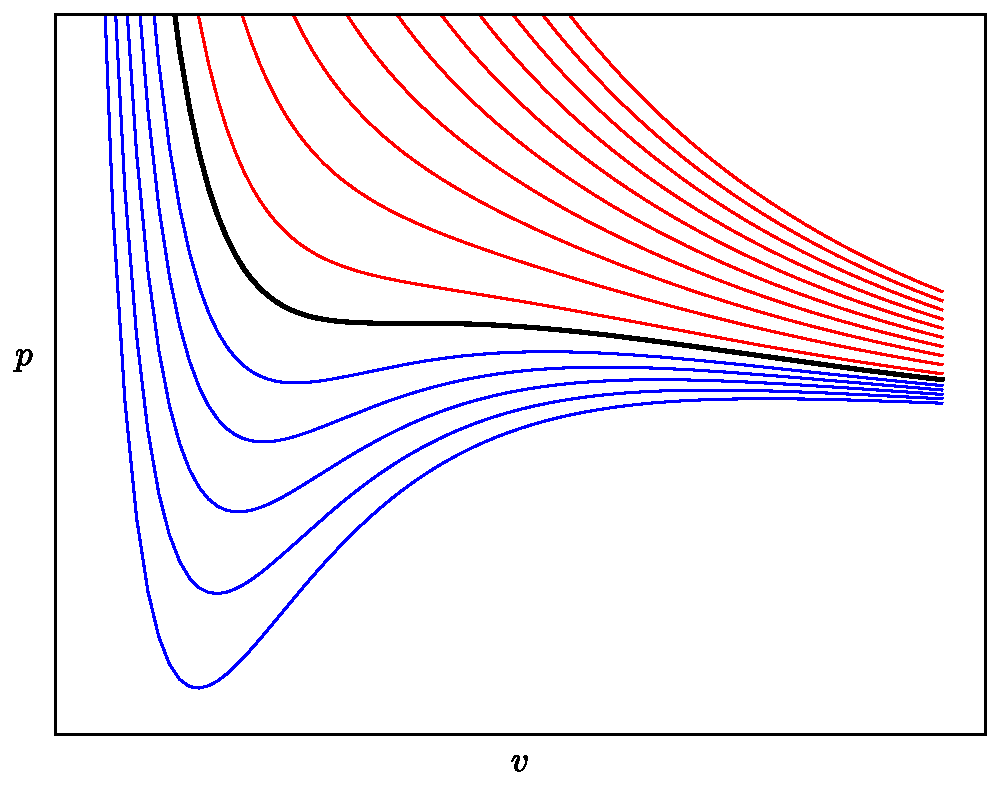
\includegraphics[width=0.75\textwidth]{Pseudopotential/vdW_isoth}
	\caption{Diagrama $p-v$ para la ecuaci\'on de van der Waals. Se destacan las isotermas supercr\'iticas (rojo), cr\'itica (negro) y subcr\'iticas (azul).}
	\label{fig:vdW_isoth}
\end{figure}

La \fig{fig:vdW_isoth} ejemplifica el comportamiento de la ecuaci\'on de van der Waals, donde cada l\'inea corresponde a una isoterma. A medida que la temperatura desciende, las isotermas pasan de un comportamiento similar a un gas ideal, en la esquina superior derecha de la figura, a exhibir un comportamiento en forma de S con un m\'inimo y un m\'aximo locales, en la esquina inferior izquierda. De acuerdo a esas isotermas, existen tres valores de densidad asociadas a una misma presi\'on. Sin embargo, en esa zona de S existe una regi\'on donde $(\partial v / \partial \rho)_T$ es positiva, y por lo tanto se tiene compresibilidad negativa, lo que implica que esa regi\'on es inestable frente a perturbaciones de presi\'on \cite{burden_numerical_2011}.
La temperatura a partir de la cual se produce este cambio de comportamiento se conoce como temperatura cr\'tica, y es la que se ilustra con una l\'inea m\'as gruesa en la \fig{fig:vdW_isoth}. Esta isoterma presenta un punto de inflexi\'on, conocido como punto cr\'itico, sobre el que se definen propiedades caracter\'isticas de la ecuaci\'on de estado. En particular, analizando las derivadas $(\partial p / \partial v)_T = 0$ y $(\partial^2 p / \partial v^2)_T = 0$, puede encontrarse cu\'al es ese punto cr\'itico, es decir, los valores de presi\'on cr\'itica, volumen molar cr\'itico y temperatura cr\'itica que lo caracterizan:
\begin{equation}
	\begin{gathered}
		p_c = \dfrac{a}{27 b^2} \\
		v_c = 3b \\
		T_c = \dfrac{8 a}{27 R b}
	\end{gathered}
	\label{eq:vdw_param_crit}
\end{equation}

En la \fig{fig:vdW_isoth} se evidencia que para temperaturas por debajo del valor cr\'itico, dos vol\'umenes molares diferentes pueden adoptar el mismo valor de presi\'on en equilibrio $p_0$ (en realidad son 3, pero uno es inestable). Por lo tanto, puede establecerse un estado de coexistencia entre dos fases, l\'iquido y vapor, que compartan igual energ\'ia libre de Gibbs (o equivalentemente potencial qu\'imico). Esta restriccici\'on implica:
\begin{equation}
	\int_{v_l}^{v_g} \left[p_0 - p(v',T)\right] \, \mbox{d} v' = 0,
	\label{eq:maxwell_constr}
\end{equation}
donde $p_0 = p(v_l,T) = p(v_g,T)$. La \eq{eq:maxwell_constr} se conoce como regla de construcci\'on de Maxwell, y determina los vol\'umenes de coexistencia de ambas fases para una determinada temperatura. Si se realiza un cambio de variables adecuado, la \eq{eq:maxwell_constr} puede reescribirse como:
\begin{equation}
	\int_{\rho_g}^{\rho_l} \left[p_0 - p(\rho',T)\right] \dfrac{1}{\rho'} \, \mbox{d} \rho' = 0,
	\label{eq:maxwell_constr_rho}
\end{equation}
donde $p_0 = p(\rho_l,T) = p(\rho_g,T)$. Gr\'aficamente, resolver la regla de Maxwell implica encontrar los vol\'umenes para los que las \'areas sombreadas de la \fig{fig:vdW_Maxwell} sean iguales. 

\begin{figure}[ht]
	\centering
	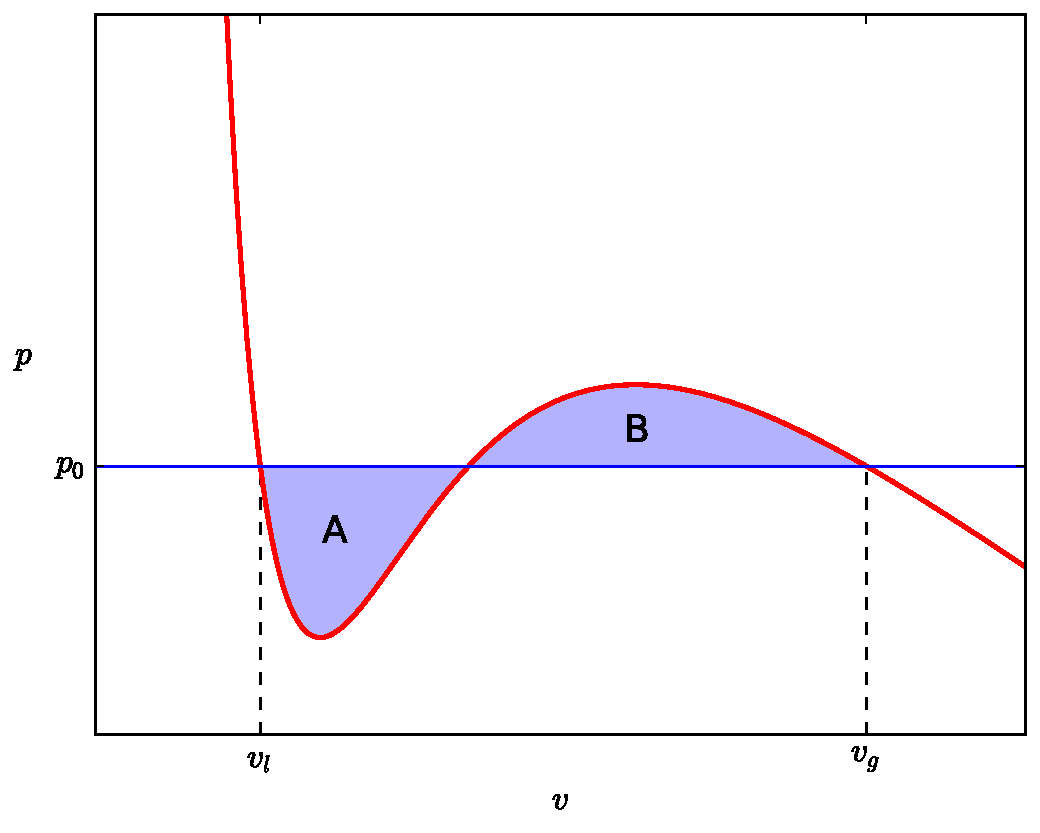
\includegraphics[width=0.75\textwidth]{Pseudopotential/vdW_Maxwell}
	\caption{Ejemplo de aplicaci\'on de la regla de construcci\'on de Maxwell. Dada una isoterma del diagrama $p-v$, los vol\'umenes de coexistencia son aquellos para los que las \'areas $A$ y $B$ son iguales.}
	\label{fig:vdW_Maxwell}
\end{figure}


La regla de construcci\'on de Maxwell aplica a cualquier ecuaci\'on de estado, e impone una restricci\'on termodin\'amica a las simulaciones realizadas con modelos pseudopotential: si se desea recuperar el comportamiento de un fluido regido por una ecuaci\'on de estado, entonces la ``separaci\'on autom\'atica de fases'' propia de esta familia debe ser capaz de reproducir las densidades de equilibrio dadas por la \eq{eq:maxwell_constr}.


\subsubsection*{Otras ecuaciones de estado}

La ecuaci\'on de estado de van der Waals ha alcanzado una notable popularidad, no s\'olo por ser la primera en modelar el comportamiento de gases reales, sino porque a pesar de su simplicidad, permite representar fen\'omenos complejos asociados a la coexistencia y cambio de fase. Sin embargo, esta ecuaci\'on no es la \'unica, ya que se ha creado un amplio abanico de posibilidades en busca de una mejor representaci\'on de diversos tipos de fluidos. A continuaci\'on se detallan dos de las m\'as conocidas, apliamente utilizadas en la literatura de lattice Boltzmann.

\smallskip
\textbf{Carnahan-Starling:}
\begin{equation}
	\begin{gathered}
		p = \rho R T\dfrac{1+b\rho/4+(b\rho/4)^2-(b\rho/4)^3}{(1-b\rho/4)^3} - a\rho^2, \\[2mm]
		p_c = \dfrac{0.07066 \, Ra}{b^2}, \\[2mm]
		T_c = \dfrac{0.37733 \, a}{Rb}, \\[2mm]
		\rho_c = \dfrac{0.5218}{b}
	\end{gathered}
\end{equation}


\textbf{Peng-Robinson:}
\begin{equation}
	\begin{gathered}
		p = \dfrac{\rho R T}{1-b\rho} - \dfrac{a\varphi(\omega,T)\rho^2}{1+2b\rho-(b\rho)^2}, \\[0mm]
		\varphi(\omega,T) = \left[ 1+(0.37464+1.54226\omega-0.26992\omega^2)(1-\sqrt{T/T_c})\right], \\[0mm]
		p_c \approx \dfrac{0.01324 \, a}{b^2}, \\[2mm]
		T_c \approx \dfrac{0.17015 \, a}{Rb}, \\[2mm]
		\rho_c \approx \dfrac{0.253077}{b}
	\end{gathered}
\end{equation}

\red{Poner ac\'a otras propiedades derivadas, como calor latente?}


\subsubsection*{Curvas de coexistencia}

Como se mencion\'o previamente, la regla de construcci\'on de Maxwell permite determinar las densidades de coexistencia en equilibrio para cualquier ecuaci\'on de estado. La determinaci\'on de los l\'imites de esta integral no siempre es sencillo, dado que requiere la aplicaci\'on de un ciclo iterativo, con resultads que dependen de las constantes caracter\'isticas de cada ecuaci\'on de estado. Este c\'alculo, as\'i como la comparaci\'on objetiva entre diferentes ecuaciones de estado, puede simplificarse si se usa el concepto de unidades reducidas \cite{mcquarrie_molecular_1999}:
\begin{equation}
	\rho_r = \rho / \rho_c, \qquad T_r = T / T_c, \qquad p_r = p / p_c,
\end{equation}
donde los sub\'indices $r$ y $c$ denotan propiedades reducidas y cr\'iticas, respectivamente. De acuerdo a la ley de estados correspondientes, las propiedades reducidas deben ser las mismas independientemente del tipo de unidades utilizadas. Por lo tanto, la relaci\'on entre propiedades de coexistencia quedan un\'ivocamente determinadas para cada ecuaci\'on de estado, si se emplean unidades reducidas. De esta forma pueden construirse las llamadas curvas universales de coexistencia, como las mostradas en la \fig{fig:EOS}.

\begin{figure}[ht]
	\centering
	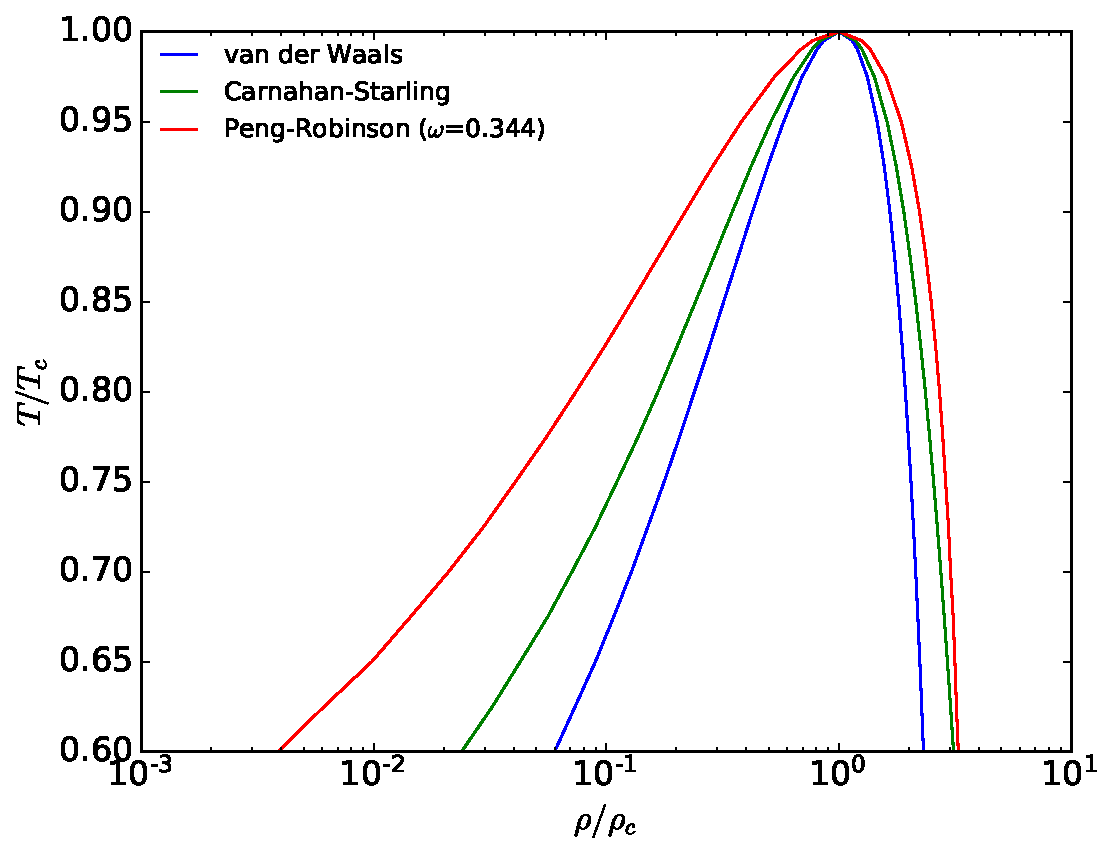
\includegraphics[width=0.75\textwidth]{Pseudopotential/EOS_comp}
	\caption{Densidades de coexistencia, en unidades reducidas, para diferentes ecuaciones de estado.}
	\label{fig:EOS}
\end{figure}





\subsection{Incorporaci\'on de ecuaciones de estado en el potencial de interacci\'on}

La definici\'on de masa efectiva dada por Shan y Chen se aproxima a un valor asint\'otico cuando la densidad es alta, lo que contribuye a evitar el colapso de la fase de mayor densidad y, por lo tanto, contribuir a mejorar la estabilidad de las simulaciones. Sin embargo, el uso de esta expresi\'on fija la ecuaci\'on de estado final, lo que limita la aplicabilidad a diferentes fluidos. En 2006. Yuan y Schaefer \cite{yuan_equations_2006} demostraron que es posible alcanzar relaciones de densidad elevadas en casos est\'aticos si se emplea la masa efectiva introducida por He y Doolen \cite{he_thermodynamic_2002}:
\begin{equation}
	\psi(\rho) = \sqrt{\dfrac{2(p_{EOS} - \rho c_s^2)}{Gc^2}},
\end{equation}
donde $p_{EOS}$ representa una ecuaci\'on de estado no ideal, como Van der Waals, Carnahan-Starling o Peng-Robinson.






\subsection{La condici\'on de estabilidad mec\'anica y el problema de inconsistencia termodn\'amica}

En el caso sin fuerzas de interacci\'on, a nivel macrosc\'opico se recupera una ecuaci\'on de estado ideal de la forma $p=\rho c_s^2$. Sin embargo, la incorporaci\'on de \ref{eq:f_int} produce una nueva ecuaci\'on de estado dependiente del potencial de interacci\'on:
\begin{equation}
	p = \rho c_s^2 + \dfrac{G}{2} c_s^2 \psi ^2,
\end{equation}
mientras que el tensor de presi\'on $\bm{P}$ queda definido como \cite{he_thermodynamic_2002}:
\begin{equation}
	\nabla \cdot \bm{P} = \nabla \cdot (\rho c_s^2 \bm{I}) - \bm{F}.
	\label{eq:ptens}
\end{equation}

Shan \cite{shan_pressure_2008} demostr\'o que para garantizar un balance mec\'anico exacto, debe considerarse una forma discreta del tensor de presi\'on. En particular, esta expresi\'on puede derivarse a partir de una integral de volumen de la \eq{eq:ptens}:
\begin{equation}
	\int (\nabla \cdot \bm{P}) \, \mbox{d}\Omega = \int \nabla \cdot (\rho c_s^2 \bm{I})\, \mbox{d}\Omega - \int \bm{F} \, \mbox{d}\Omega,
	\label{eq:integral_pres}
\end{equation}
donde $\Omega$ es un volumen cerrado. Si se aplica el teorema de integraci\'on de Gauss a la \eq{eq:integral_pres} resulta
\begin{equation}
	\int \bm{P} \, \mbox{d} \bm{A} = \int \rho c_s^2 \bm{I}\, \mbox{d} \bm{A} - \int \bm{F} \, \mbox{d}\Omega,
\end{equation}
donde $\mbox{d} \bm{A}$ es un diferencial de \'area. En forma discreta, esta integral puede escribirse como
\begin{equation}
	\sum \bm{P} \cdot \bm{A} = \sum \rho c_s^2 \bm{I} \cdot \bm{A} - \sum \bm{F}.
\end{equation}

Por lo tanto, el tensor de presi\'on finalmente puede escribirse como:
\begin{equation}
	\bm{P} = \rho c_s^2 \bm{I} + \dfrac{G}{2}\psi(\bm{x}) \sum_{\alpha=1}^N w(|\bm{e}_{\alpha}|^2)\psi(\bm{x}+\bm{e}_{\alpha})\bm{e}_{\alpha}\bm{e}_{\alpha}.
	\label{eq:ptens_shan}
\end{equation}

En el caso de considerar s\'olo interacciones con los vecinos cercanos (ubicados a una distancia m\'axima de $\sqrt{2}$ o $\sqrt{3}$ unidades de grilla en 2 o 3 dimensiones respectivamente), la expansi\'on en serie de Taylor de la \eq{eq:ptens_shan} resulta:
\begin{equation}
	\bm{P} = \left( \rho c_s^2 + \dfrac{G c^2}{2} \psi^2 + \dfrac{G c^4}{12} \psi \nabla^2 \psi \right) \bm{I} + \dfrac{G c^4}{6} \psi \nabla \nabla \psi.
	\label{eq:ptens_shan_taylor}	
\end{equation}

La \eq{eq:ptens_shan_taylor} puede usarse para determinar la presi\'on normal a una interfase plana
\begin{equation}
	P_n = \rho c_s^2 + \dfrac{G c^2}{2} \psi^2 + \dfrac{G c^4}{12} \left[ \alpha \left( \dfrac{d\psi}{dn} \right)^2 + \beta \psi \dfrac{d^2 \psi}{dn^2} \right],
	\label{eq:ptens_shan_plane}	
\end{equation}
donde $n$ denota la direcci\'on normal a la interfase, y en el caso de interacci\'on de vecinos cercanos se cumple $\alpha = 0$ y $\beta = 3$. Por lo tanto, tomando como base la \eq{eq:ptens_shan_plane} y considerando que en equilibrio la presi\'on $P_n$ debe ser igual a la presi\'on est\'atica en el seno del fluido \cite{shan_pressure_2008}, puede derivarse la condici\'on de estabilidad mec\'anica:
\begin{equation}
	\int_{\rho_g}^{\rho_l} \left( p_0 - \rho c_s^2 - \dfrac{Gc^2}{2} \psi^2 \right) \dfrac{\psi'}{\psi^{1+\varepsilon}} \, \mbox{d}\rho = 0,
\end{equation}
donde $\psi' = d\psi / d\rho$, $\varepsilon=-2\alpha/\beta$ y $p_0=p(\rho_l)=p(\rho_g)$. De esta forma, puede verse que la condici\'on de estabilidad mec\'anica conduce a densidades de coexistencia que en general ser\'an diferentes a las establecidas por la construcci\'on de Maxwell (\eq{eq:maxwell_constr_rho}), ya que si el potencial de interacci\'on satisface la propuesta de He y Doolen, entonces en general no puede cumplirse que $\psi' / \psi^{1+\varepsilon} \propto 1/\rho^2$. Esta incompatibilidad se conoce con el nombre de inconsistencia termodin\'amica.


\section{El modelo isot\'ermico de Li et al.}


